\documentclass[a4paper, 12pt]{article}
\usepackage[a4paper, total={6in, 9.5in}]{geometry} % DL: 쪽여백 조정
\usepackage{setspace} % DL: 줄간격 조정
\usepackage{graphicx} % Required for inserting images
\usepackage{kotex}
\usepackage{amsmath,amsthm,amssymb,amsfonts,mdframed}

% set indent length to zero.
\setlength{\parindent}{0pt}

\title{1002 Class Activity}
\author{박예영}

\begin{document}
\maketitle
\begin{mdframed}
Find $\chi (G)$ and $\chi ' (G)$ for these $3$ graphs.
\centering
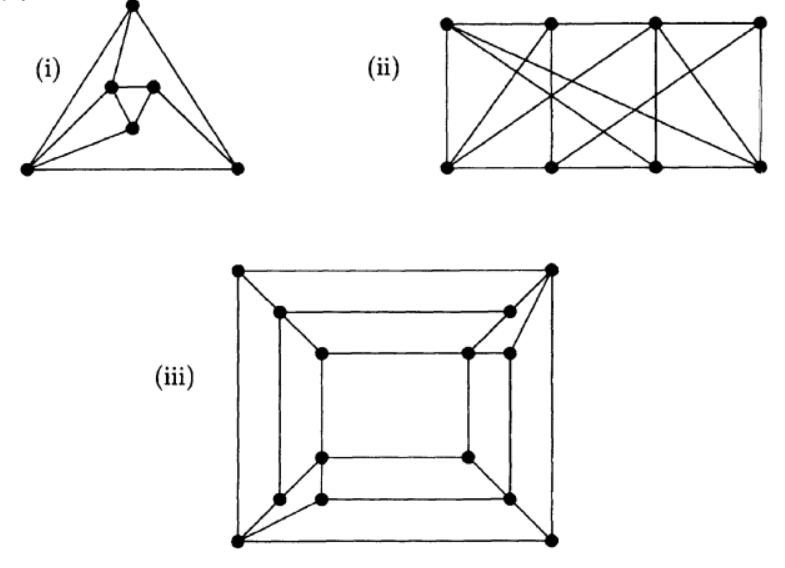
\includegraphics[width=0.5\linewidth]{image1.png}
\end{mdframed}
\doublespacing

\begin{proof}

(i) \\
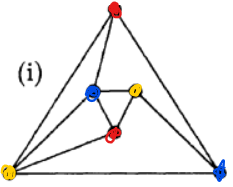
\includegraphics[width=0.25\linewidth]{image2.png} \\
By this vertex coloring, we can claim that $\chi (G) \leq 3$. \\
It is obvious that $\chi (G) \neq 1$. \\
If $\chi (G) = 2$, all vertices incident with the top red vertex must be the same color. Let this color "Blue". However, the left blue vertex and the right blue vertex are incident each other, so, we cannot color like this way. Therefore, $\chi (G) = 3$. \\
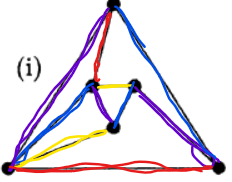
\includegraphics[width=0.25\linewidth]{image3.png} \\
By this edge coloring, we can claim that $\chi '(G) \leq 4$.\\ 
By Vizing's Theorem, $\chi '(G) = \Delta \textrm{ or } \Delta + 1 = 4 \textrm{ or } 5$. Therefore, $\chi '(G) = 4$. \\

(ii) \\
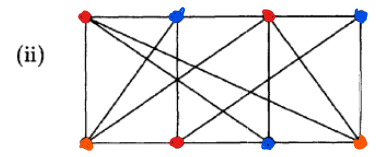
\includegraphics[width=0.5\linewidth]{image4.png} \\
By this vertex coloring, we can claim that $\chi (G) \leq 3$. \\
It is obvious that $\chi (G) \neq 1$. \\ 
If $\chi (G) = 2$, all vertices incident with the top left red vertex must be the same color. Let this color "Orange". However, the bottom left orange vertex and the top second left orange vertex are incident each other, so, we cannot color like this way. Therefore, $\chi (G) = 3$. \\
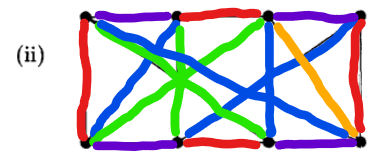
\includegraphics[width=0.5\linewidth]{image5.png} \\
By this edge coloring, we can claim that $\chi '(G) \leq 5$. \\
We know that $\chi '(G) \geq \Delta$, where $\Delta$ is the maximum vertex degree of graph $G$ and $\Delta (G) = 5$, therefore, $\chi '(G) = 5$. \\

(iii) \\
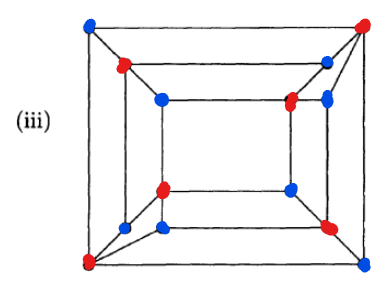
\includegraphics[width=0.5\linewidth]{image6.png} \\
By this vertex coloring, we can claim that $\chi (G) \leq 2$, also, it is obvious that $\chi (G) \neq 1$ since there are incident vertices. Hence, $\chi (G) = 2$, which means it is "Bipartite Graph". Because $G$ is "Bipartite graph", we can claim that $\chi '(G) = \Delta (G) = 4$.
\end{proof}

\end{document}
